En latch, eller flip-flop, er en 1bit minne.
Den kan lagre en enkel tilstand, av eller på.
Et større minne settes sammen av flere flip-flops.



\paragraph{SR-latch} \mbox{} \\
Den enkleste latchen består av to input og to output.
\\\\
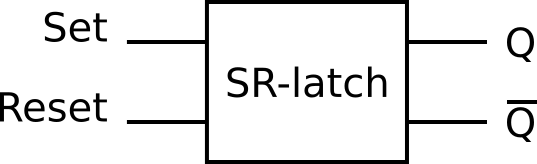
\includegraphics[width=0.5\textwidth]{./img/sr-latch}
TODO: Forklar



\paragraph{$\overline{SR}$-latch} \mbox{} \\
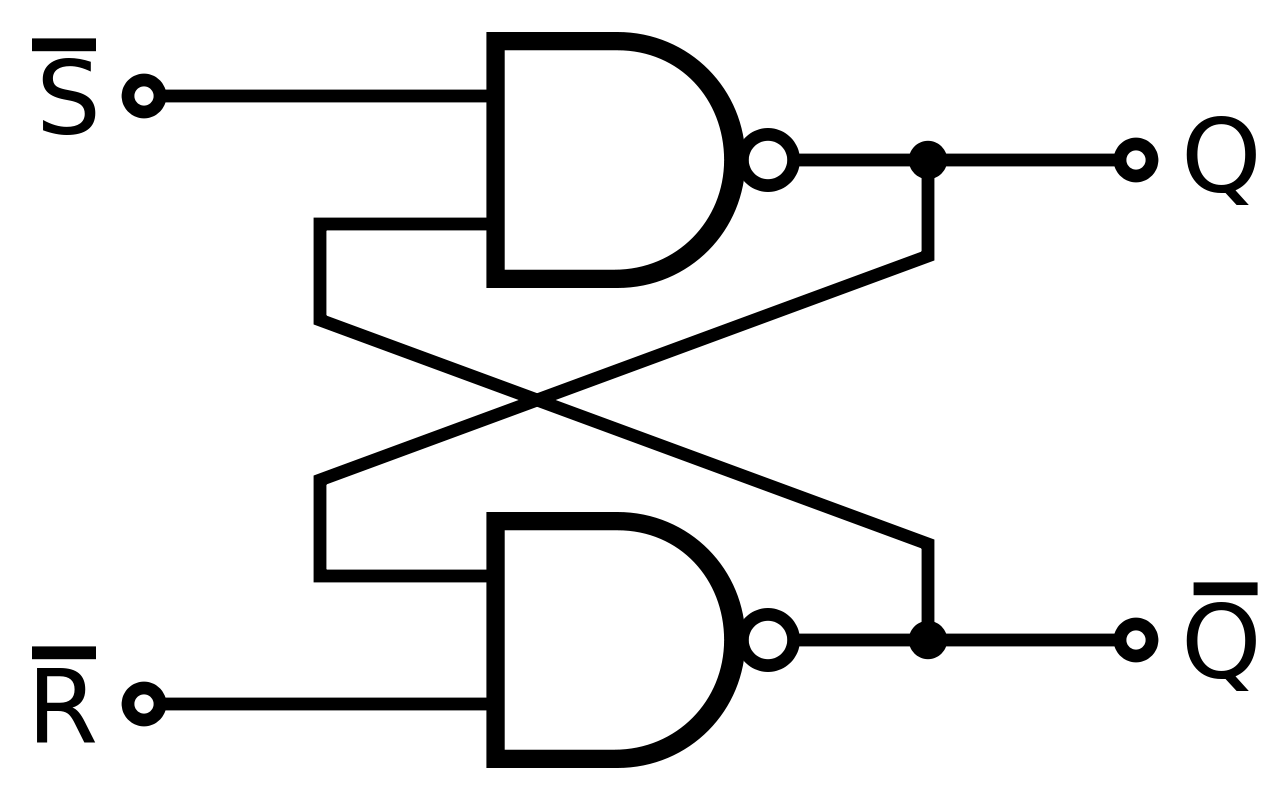
\includegraphics[width=0.5\textwidth]{./img/not-sr}
\\\\
TODO: Forklar og sannhetstabell



\paragraph{Synkron SR-latch} \mbox{} \\
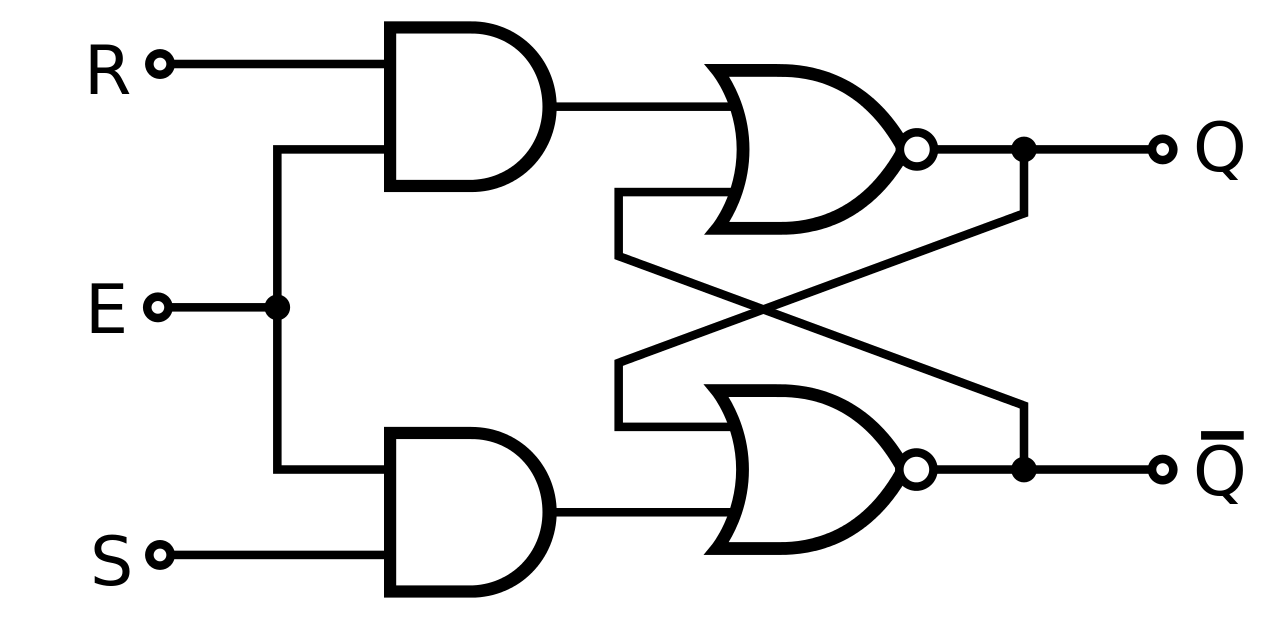
\includegraphics[width=0.67\textwidth]{./img/klokket-sr}
\\\\
TODO



\paragraph{D-latch} \mbox{} \\
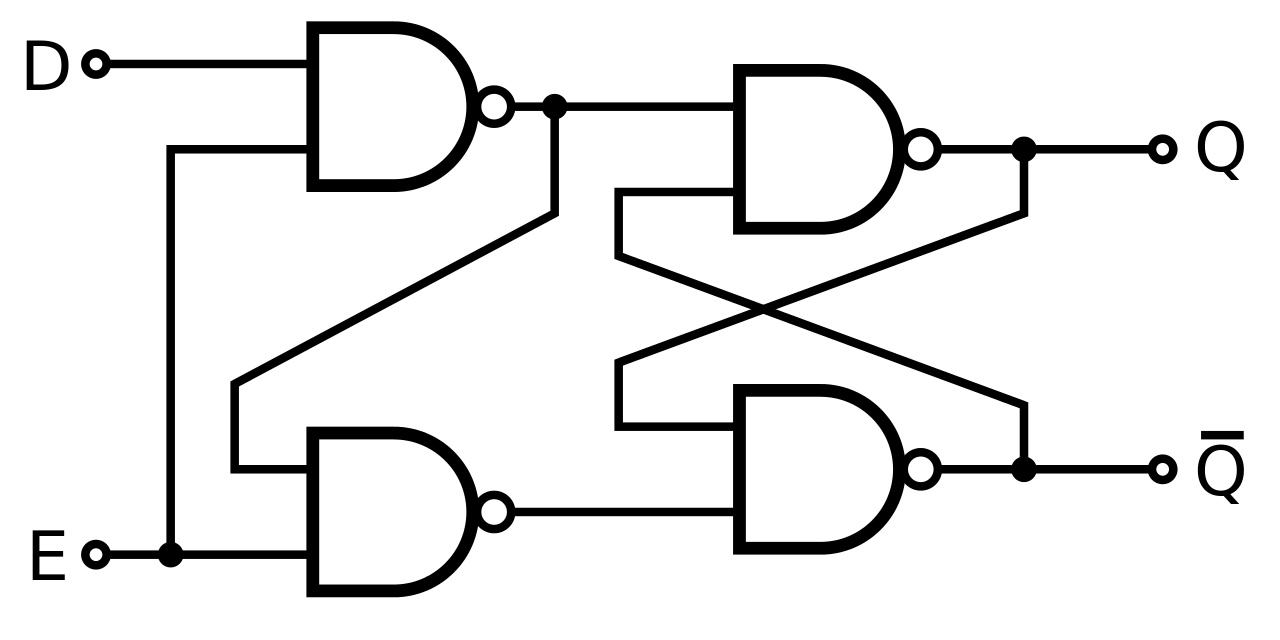
\includegraphics[width=0.67\textwidth]{./img/klokket-dlatch}
\\\\
TODO
